\documentclass{beamer}
\usepackage{mathtools}
\usepackage{amsmath}
\usepackage{datetime}

\mode<presentation>{\usetheme{Warsaw}}

% --- Color Customization Start ---
\usepackage[T1]{fontenc}
\usepackage[utf8]{inputenc}
\usepackage{xcolor}
\definecolor{myburgundy}{RGB}{172,0,52} %Add the ID of color
\setbeamercolor{structure}{fg=myburgundy}
\setbeamercolor{section in head/foot}{fg=myburgundy}
\setbeamercolor{subsection in head/foot}{fg=myburgundy}
\setbeamercolor{author in head/foot}{fg=myburgundy}
\setbeamercolor{title in head/foot}{fg=myburgundy}
\setbeamercolor{date in head/foot}{fg=myburgundy}

% Code command background
\usepackage{inconsolata}      % nicer monospace
\usepackage[many]{tcolorbox}  % inline boxes with rounded corners
\newtcbox{\icode}{on line,
  boxsep=0.6pt, left=2pt, right=2pt, top=1pt, bottom=1pt,
  colback=gray!15, colframe=gray!30, boxrule=0.4pt,
  enhanced, arc=2pt, outer arc=2pt}

% Listings for code
\usepackage{listings}
\lstset{
  language=Python,
  basicstyle=\ttfamily\small,
  keywordstyle=\rmfamily\bfseries,
  showstringspaces=false,
  columns=fullflexible,
  frame=single,
  breaklines=true
}
% --- Color Customization End ---
\usepackage{braket} % \bra{}, \ket{}, \braket{}, \ketbra{}
\newcommand{\ketbra}[2]{\ket{#1}\!\bra{#2}}
\usepackage[english]{babel}
\usepackage{bm}
\usepackage{tikz}
\usebackgroundtemplate{%
\tikz[overlay,remember picture] \node[opacity=0.10, at=(current page.center)] {
  
\includegraphics[width=2.5in]{Figures/FPTU_logo.png}};}
\usepackage{amsmath}
\usepackage{adjustbox}
\usepackage{times}
\usepackage{subfig}
\usepackage{graphicx}
\usepackage{epstopdf}
\usepackage{multirow}
\usepackage{booktabs}
\usepackage{orcidlink}
\useoutertheme{infolines}
\setbeamertemplate{itemize items}[ball]
\setbeamertemplate{itemize subitem}[square]
\setbeamertemplate{itemize subsubitem}[triangle]
\setbeamertemplate{enumerate items}[default]
\setbeamertemplate{footline}
{
  \leavevmode%
  \hbox{%
  \begin{beamercolorbox}[wd=.23\paperwidth,ht=2.25ex,dp=1ex,center]{author in head/foot}%
    \usebeamerfont{author in head/foot}\insertshortauthor
  \end{beamercolorbox}%
  \begin{beamercolorbox}[wd=.62\paperwidth,ht=2.25ex,dp=1ex,center]{title in head/foot}%
    \usebeamerfont{subsection in head/foot}\insertshorttitle
  \end{beamercolorbox}%
  \begin{beamercolorbox}[wd=.15\paperwidth,ht=2.25ex,dp=1ex,center]{date in head/foot}%
    \insertframenumber{}/\inserttotalframenumber 
  \end{beamercolorbox}}%
  \vskip0pt%
}

\makeatletter
\setbeamertemplate{headline}
{%
  \leavevmode%
  \@tempdimb=2.6575ex%
  \ifnum\beamer@subsectionmax<\beamer@sectionmax%
    \multiply\@tempdimb by\beamer@sectionmax%
  \else%
    \multiply\@tempdimb by\beamer@subsectionmax%
  \fi%
  \ifdim\@tempdimb>0pt%
    \advance\@tempdimb by 1.825ex%
    \begin{beamercolorbox}[wd=.5\paperwidth,ht=\@tempdimb]{section in head/foot}%
      \vbox to\@tempdimb{\vfil\insertsectionnavigation{.5\paperwidth}\vfil}%
    \end{beamercolorbox}%
    \begin{beamercolorbox}[wd=.5\paperwidth,ht=\@tempdimb]{subsection in head/foot}%
      \vbox to\@tempdimb{\vfil\insertsubsectionnavigation{.5\paperwidth}\vfil}%
    \end{beamercolorbox}%
  \fi%
}
\makeatother
\newdate{mydate}{25}{09}{2025}
\title[\textbf{Single and Multiple qubits System}]
{\textbf{Quantum Fundamentals: Single and Multiple Qubit Systems}}
\author[Nguyen Minh Tri]
{Presenter: Nguyen Minh Tri}
\date[\displaydate{mydate}]{ 
\small \textcolor{myburgundy}{\textbf{Quantum Seminar} \\ \displaydate{mydate}}}

\begin{document}
\begin{frame}[plain]
  \titlepage
\end{frame}

\begin{frame}[allowframebreaks]{Outline}
    \tableofcontents
\end{frame}

\section{Complex number}
\subsection{Why must it be a complex number?}

\begin{frame}[fragile]{The Qubit State \& The Necessity of Complex Numbers}
    \begin{block}{Premise: Quantum States Have Wave-like Properties}
        As established, quantum systems behave like waves. A key property of any wave is its \textbf{phase}. Therefore, our mathematical description of a quantum state must be able to account for this phase.
    \end{block}
    
    \begin{block}{The General State of a Qubit}
        The most general way to write the state of a single qubit, $|\psi\rangle$, is:
        \[|\psi\rangle = \cos\frac{\theta}{2}|0\rangle + e^{i\phi}\sin\frac{\theta}{2}|1\rangle\]
        \begin{itemize}
            \item The real parts control the \textbf{probability balance} between $\ket{0}$ and $\ket{1}$.
            \item The term $e^{i\phi}$ is the crucial \textbf{relative phase factor}.
        \end{itemize}
    \end{block}
\end{frame}

\begin{frame}[fragile]{Why Complex Numbers are Essential}
    \begin{alertblock}{The Nature of the Phase Factor (Euler's Formula)}
        The phase factor is defined by Euler's formula, which is inherently complex:
        \[
        e^{i\phi} = \cos(\phi) + i\sin(\phi)
        \]
        \textbf{Conclusion:} To fully describe a qubit's state, we must include its relative phase ($e^{i\phi}$). Since this phase factor is fundamentally a complex number (containing $i$), the entire framework for describing quantum states \textbf{must use complex numbers}.
    \end{alertblock}
\end{frame}

\section{Hilbert Space of Multi-Qubit Systems}
\begin{frame}[fragile]{Combining Hilbert Spaces: The Tensor Product}
    How do we mathematically describe a two-qubit system? We combine their spaces using the \textbf{tensor product} ($\otimes$).

    \begin{block}{Rule: Forming the New Basis}
        The basis for the combined system is formed by the tensor product of \textbf{every} basis vector from each individual space.
        \begin{itemize}
            \item Qubit A basis: $\{ \ket{0}_A, \ket{1}_A \}$
            \item Qubit B basis: $\{ \ket{0}_B, \ket{1}_B \}$
        \end{itemize}
        
        The new 4D basis for the combined system is:
        \[ \{ \ket{00}, \ket{01}, \ket{10}, \ket{11} \} \]
    \end{block}
\end{frame}

\begin{frame}[fragile]{Tensor Product: Vector Representation}
    \begin{block}{Example: Kronecker Product}
        The tensor product of column vectors is the \textbf{Kronecker product}:
        \[
        \ket{01} = \ket{0} \otimes \ket{1} = \begin{pmatrix} 1 \\ 0 \end{pmatrix} \otimes \begin{pmatrix} 0 \\ 1 \end{pmatrix} = \begin{pmatrix} 0 \\ 1 \\ 0 \\ 0 \end{pmatrix}
        \]
        This is why the Hilbert space dimensions multiply: $2 \times 2 = 4$.
    \end{block}
\end{frame}

\section{Core Concepts Revisited}
\subsection{Superposition}

% --- Slide này giữ nguyên, đã tốt ---
\begin{frame}[fragile]{Superposition: The Fundamental Rule}
    \begin{block}{The "Rule of the Game"}
        The principle of superposition is a direct consequence of the linearity of the Schrödinger equation in Hilbert space.
    \end{block}

    \begin{itemize}
        \item \textbf{Core Idea:} If a system can be in state $\ket{A}$ and also in state $\ket{B}$, then any linear combination $\ket{\psi} = \alpha\ket{A} + \beta\ket{B}$ is also a valid state.
        
        \item \textbf{Wave Analogy:} Multiple individual waves adding up to form a single composite wave, allowing for interference.
    \end{itemize}
\end{frame}

\begin{frame}[fragile]{Superposition: Visual Example}
    \begin{figure}
        \centering
        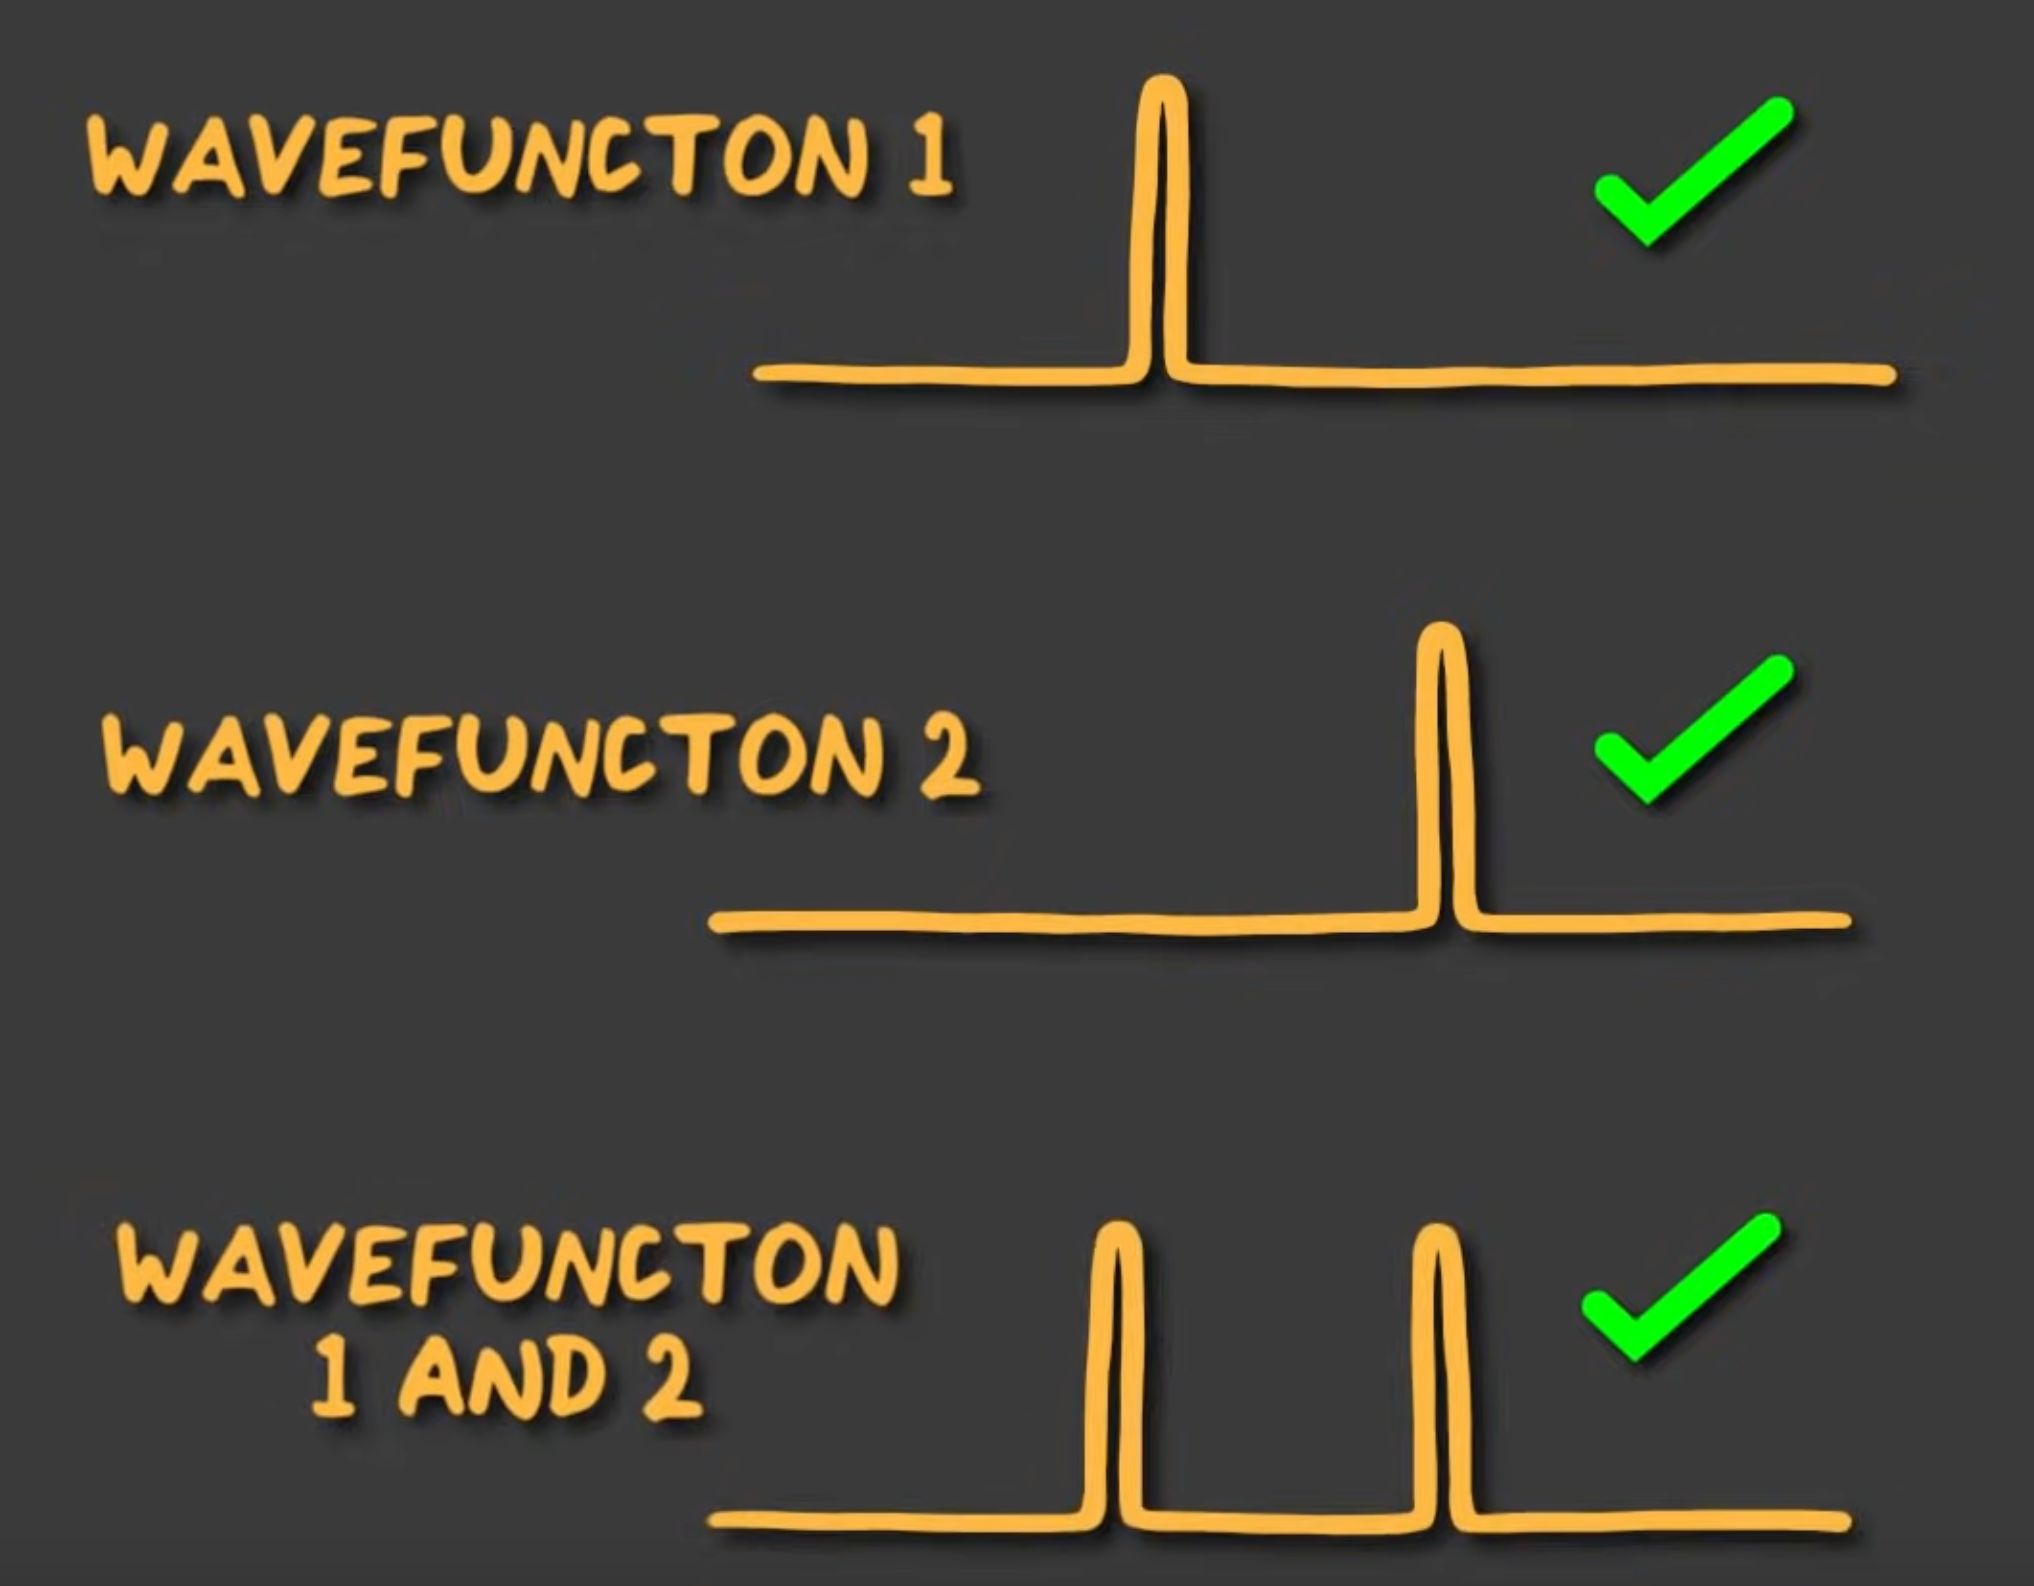
\includegraphics[width=0.6\linewidth]{Figures/Superposition.png}
        \caption{Combination of 2 wave functions}
        \label{fig:placeholder}
    \end{figure}
    
    \textbf{For a Qubit:} This is why a qubit's state can be $\ket{\psi} = \alpha\ket{0} + \beta\ket{1}$.
\end{frame}

\subsection{Entanglement}

% --- Slide "Entanglement" được tách thành 4 slide riêng biệt ---

\begin{frame}[fragile]{Entanglement: The Essence}
    \begin{block}{What is an Entangled State?}
        An entangled state is a shared state for a multi-part system that \textbf{cannot be separated} into individual states for its components.
        \begin{itemize}
            \item \textbf{Separable State:} $\ket{01} = \ket{0} \otimes \ket{1}$.
            \newline (We can describe each qubit individually).
            \item \textbf{Entangled State:} $\frac{1}{\sqrt{2}}(\ket{00} + \ket{11})$.
            \newline (The state of one qubit is undefined without the other).
        \end{itemize}
    \end{block}
\end{frame}

\begin{frame}[fragile]{Entanglement vs. Our Classical Worldview}
    \begin{block}{Our Intuition: Local Realism}
        For centuries, physics was built on two intuitive assumptions:
        \begin{enumerate}
            \item \textbf{Realism:} Objects have definite, pre-existing properties, independent of observation.
            \newline\textit{(A hidden coin is already heads or tails; we just don't know which.)}
            
            \item \textbf{Locality:} An object is only influenced by its immediate surroundings. No influence can travel faster than light.
            \newline\textit{(Flipping a coin here cannot instantly flip a coin on the Moon.)}
        \end{enumerate}
    \end{block}

    \begin{alertblock}{The "Spooky" Challenge}
        Entanglement seems to violate this. Measuring one particle appears to instantly determine the state of its distant partner.
    \end{alertblock}
\end{frame}

\begin{frame}[fragile]{The Verdict: Bell's Theorem}
    \begin{block}{The Decisive Test}
        \begin{itemize}
            \item In 1964, John Bell devised a mathematical test. He proved that if local realism were true, the correlations between entangled particles would have a strict limit.
            \item \textbf{Experiments have decisively and repeatedly shown that this limit is violated.}
        \end{itemize}
    \end{block}
    
    \begin{exampleblock}{Conclusion: Reality is Weirder Than We Think}
        The universe does \textbf{not} obey Local Realism. We must abandon at least one of our core classical assumptions about reality.
        \\Bell's Inequality: \url{https://www.youtube.com/watch?v=9OM0jSTeeBg}
    \end{exampleblock}
\end{frame}

\begin{frame}[fragile]{Making Sense of It: The Many-Worlds Interpretation}
    \begin{block}{One Possible "Story": The Branching Universe}
        This is a mathematically elegant and increasingly popular interpretation to explain the strangeness of entanglement.
        \begin{itemize}
            \item \textbf{Core Idea:} The wave function is real and never collapses. Instead, the universe \textbf{branches} for each possible measurement outcome.
            \item \textbf{How it explains entanglement:}
            \begin{itemize}
                \item When you measure your entangled qubit, the universe splits. 
                \item In one branch, you get 0 and your distant partner also gets 0.
                \item In another branch, another "you" gets 1 and your partner gets 1.
                \item The perfect correlation is preserved across corresponding branches. The "spooky action" is the branching of reality itself.
            \end{itemize}
        \end{itemize}
    \end{block}
\end{frame}
\section{Qubit Mathematics \& Single-Qubit Gates}

\subsection{Single-Qubit Gates}
\begin{frame}[fragile]{Single-Qubit Gates: Unitary Operations}
    \begin{itemize}
        \item \textbf{Overview:} Gates are 2x2 unitary matrices acting on qubit state: $|\psi'\rangle = U |\psi\rangle$, with $U^\dagger U = I$.
    \end{itemize}
\end{frame}

\begin{frame}[fragile]{Pauli Gates}
    \begin{itemize}
        \item \textbf{Pauli-X (NOT/bit-flip):} 
        \[ X = \begin{pmatrix} 0 & 1 \\ 1 & 0 \end{pmatrix} \]
        Flips $\ket{0}$ to $\ket{1}$ and $\ket{1}$ to $\ket{0}$.
        \item \textbf{Pauli-Z (phase flip):} 
        \[ Z = \begin{pmatrix} 1 & 0 \\ 0 & -1 \end{pmatrix} \]
        Leaves $\ket{0}$ unchanged, flips phase of $\ket{1}$ to $-\ket{1}$.
        \item \textbf{Pauli-Y (bit + phase flip):} 
        \[ Y = \begin{pmatrix} 0 & -i \\ i & 0 \end{pmatrix} \]
        Combines effects of X and Z.
    \end{itemize}
\end{frame}

\begin{frame}[fragile]{Hadamard (H) Gate}
    \begin{itemize}
        \item \textbf{Superposition Creator:} 
        \[ H = \frac{1}{\sqrt{2}} \begin{pmatrix} 1 & 1 \\ 1 & -1 \end{pmatrix} \]
        \item \textbf{Examples:}
        \begin{itemize}
            \item $H|0\rangle = \frac{1}{\sqrt{2}} (|0\rangle + |1\rangle) = \ket{+}$ (equal probabilities for 0 and 1).
            \item $H|1\rangle = \frac{1}{\sqrt{2}} (|0\rangle - |1\rangle) = \ket{-}$.
        \end{itemize}
    \end{itemize}
\end{frame}

\begin{frame}[fragile]{Phase Gates}
    \begin{itemize}
        \item \textbf{General Phase Gate ($P_{\theta}$):}
        \[ P_{\theta} = \begin{pmatrix} 1 & 0 \\ 0 & e^{i \theta}\end{pmatrix} \]
        Leaves $\ket{0}$ unchanged, applies a phase $e^{i\theta}$ to $\ket{1}$.
        \item \textbf{S Gate:} A specific phase gate where $\theta = \frac{\pi}{2}$.
        \[ S = P_{\frac{\pi}{2}} = \begin{pmatrix} 1 & 0 \\ 0 & i\end{pmatrix} \]
        \item \textbf{T Gate:} A specific phase gate where $\theta = \frac{\pi}{4}$.
        \[ T = P_{\frac{\pi}{4}} = \begin{pmatrix} 1 & 0 \\ 0 & \frac{1+i}{\sqrt{2}}\end{pmatrix} \]
    \end{itemize}
\end{frame}

\subsection{Rotation Gates}
\begin{frame}[fragile]{Rotation Gates: Why We Need Them}
    \begin{block}{Continuous Control}
        \begin{itemize}
            \item Unlike Pauli gates (fixed 0/1 flips or 90/180-degree phase shifts), rotation gates allow \textbf{continuous control} over the qubit's state.
            \item Essential for fine-tuning quantum states and implementing algorithms that require parameter optimization.
        \end{itemize}
    \end{block}
    
    \begin{alertblock}{Visualization}
        All single-qubit rotations can be visualized as rotating the state vector on the \textbf{Bloch Sphere}.
        \newline \href{https://bloch.kherb.io/}{\textcolor{blue}{Interactive Bloch Sphere Visualizer}}
    \end{alertblock}
\end{frame}

\begin{frame}[fragile]{Rotation Gates: X and Y Rotations}
    \begin{itemize}
        \item \textbf{Rotation around X-axis (RX($\theta$)):}
        \[ R_x(\theta) = \begin{pmatrix} \cos(\theta/2) & -i\sin(\theta/2) \\ -i\sin(\theta/2) & \cos(\theta/2) \end{pmatrix} \]
        
        \item \textbf{Rotation around Y-axis (RY($\theta$)):}
        \[ R_y(\theta) = \begin{pmatrix} \cos(\theta/2) & -\sin(\theta/2) \\ \sin(\theta/2) & \cos(\theta/2) \end{pmatrix} \]
    \end{itemize}
\end{frame}

\begin{frame}[fragile]{Rotation Gates: Z Rotation}
    \begin{itemize}
        \item \textbf{Rotation around Z-axis (RZ($\theta$)):}
        \[ R_z(\theta) = \begin{pmatrix} e^{-i\theta/2} & 0 \\ 0 & e^{i\theta/2} \end{pmatrix} \]
        
        \item Rotates the state vector around the Z-axis by an angle $\theta$.
        \item This gate primarily affects the phase of the $\ket{1}$ component.
    \end{itemize}
\end{frame}

\subsection{Single-Qubit Calculations}
\begin{frame}[fragile]{Single-Qubit Calculations: Matrix Multiplication}
    \begin{itemize}
        \item \textbf{Goal:} Apply $X$, then $H$ on $|0\rangle$, compute via matrices.
        \item \textbf{Step 1 (X Gate):} $X = \begin{pmatrix} 0 & 1 \\ 1 & 0 \end{pmatrix}$, $X |0\rangle = \begin{pmatrix} 0 & 1 \\ 1 & 0 \end{pmatrix} \begin{pmatrix} 1 \\ 0 \end{pmatrix} = \begin{pmatrix} 0 \\ 1 \end{pmatrix} = |1\rangle$.
        \item \textbf{Step 2 (H Gate):} $H = \frac{1}{\sqrt{2}} \begin{pmatrix} 1 & 1 \\ 1 & -1 \end{pmatrix}$, 
        \[
        H |1\rangle = \frac{1}{\sqrt{2}} \begin{pmatrix} 1 & 1 \\ 1 & -1 \end{pmatrix} \begin{pmatrix} 0 \\ 1 \end{pmatrix} = \frac{1}{\sqrt{2}} \begin{pmatrix} 1 \\ -1 \end{pmatrix} = \frac{|0\rangle - |1\rangle}{\sqrt{2}} = |-\rangle.
        \]
    \end{itemize}
\end{frame}

\begin{frame}[fragile]{Single-Qubit Calculations: Combined Operation}
    \begin{itemize}
        \item \textbf{Combined Matrix:} To get the final state, we multiply the gate matrices in reverse order of application (right to left on the circuit diagram).
        \[ U = H \cdot X =  \frac{1}{\sqrt{2}} \begin{pmatrix} 1 & 1 \\ 1 & -1 \end{pmatrix} \begin{pmatrix} 0 & 1 \\ 1 & 0 \end{pmatrix} = \frac{1}{\sqrt{2}} \begin{pmatrix} 1 & 1 \\ -1 & 1 \end{pmatrix} \]
        \item \textbf{Final State:} Applying the combined matrix $U$ to the initial state $|0\rangle$:
        \[
        U |0\rangle = \frac{1}{\sqrt{2}} \begin{pmatrix} 1 & 1 \\ -1 & 1 \end{pmatrix} \begin{pmatrix} 1 \\ 0 \end{pmatrix} = \frac{1}{\sqrt{2}} \begin{pmatrix} 1 \\ -1 \end{pmatrix} = |-\rangle.
        \]
    \end{itemize}
\end{frame}

\section{Two-Qubit Systems}
\subsection{Two-Qubit Systems}
\begin{frame}[fragile, allowframebreaks]{Two-Qubit Systems: State Space}
    \begin{itemize}
        \item \textbf{Why Multi-Qubits?}
        \begin{itemize}
            \item Single qubit: 2D Hilbert space ($\ket{\psi} = \alpha \ket{0} + \beta \ket{1}$).
            \item Two qubits: 4D Hilbert space via tensor product, which enables entanglement.
        \end{itemize}
        \bigskip
        \item \textbf{Tensor Product ($\otimes$):} Combines individual state spaces.
        \begin{itemize}
            \item Example: $\ket{0} \otimes \ket{0} = \ket{00} = \begin{pmatrix} 1 \\ 0 \\ 0 \\ 0 \end{pmatrix}$.
        \end{itemize}
        \bigskip
        \item \textbf{General State:} A superposition of all 4 basis states.
        \[ \ket{\Psi} = a \ket{00} + b \ket{01} + c \ket{10} + d \ket{11} \]
        With normalization: $|a|^2 + |b|^2 + |c|^2 + |d|^2 = 1$.
    \end{itemize}
\end{frame}

\begin{frame}[fragile, allowframebreaks]{Two-Qubit Systems: Multi-Qubit Gates}
    \begin{block}{Example: Apply H on the first qubit}
        To apply a Hadamard gate to the first qubit while leaving the second unchanged ($I$), we use the tensor product of the gate matrices: $H \otimes I$.
        \vspace{1em}
        The resulting 4x4 matrix is:
        \[
        H \otimes I = \frac{1}{\sqrt{2}} \begin{pmatrix} 1 & 0 & 1 & 0 \\ 0 & 1 & 0 & 1 \\ 1 & 0 & -1 & 0 \\ 0 & 1 & 0 & -1 \end{pmatrix}
        \]
        \vspace{1em}
    \end{block}
    \begin{block}{Applying}
        Applying this to the state $\ket{00}$:
        \[ 
        (H \otimes I) \ket{00} = \frac{\ket{00} + \ket{10}}{\sqrt{2}}
        \]
        This creates a superposition between the two qubits.
    \end{block}
\end{frame}

\begin{frame}[fragile, allowframebreaks]{Example Calculation On Circuit}
    \begin{figure}
        \centering
        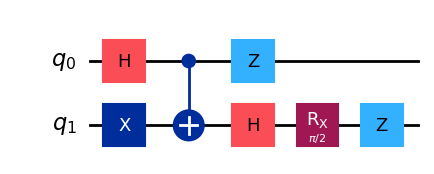
\includegraphics[width=0.7\linewidth]{Figures/Sample_circuit.png}
        \caption{Sample Circuit: Two-Qubit Circuit with Multiple Gates}
    \end{figure}
    
    \begin{block}{Circuit Operations}
        \begin{itemize}
            \item Qubit 0: $H \rightarrow Z$
            \item Qubit 1: $X \rightarrow H \rightarrow R_X(\pi/2) \rightarrow Z$
            \item CNOT between qubits
        \end{itemize}
        \textbf{Initial:} $|\psi_0\rangle = |00\rangle$
    \end{block}
    
    \framebreak
    \begin{figure}
        \centering
        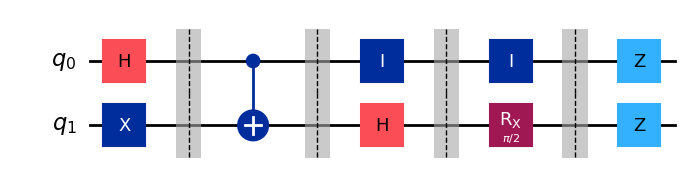
\includegraphics[width=0.8\linewidth]{Figures/circuit_clarify.png}
        \caption{Clarified Circuit with Gate Labels}
    \end{figure}

    \framebreak
    
    \begin{block}{Step 1: Define Gate Matrices}
        \textbf{Single-qubit gates:}
        \[
        H = \frac{1}{\sqrt{2}} \begin{pmatrix} 1 & 1 \\ 1 & -1 \end{pmatrix}, \quad
        X = \begin{pmatrix} 0 & 1 \\ 1 & 0 \end{pmatrix}, \quad
        I = \begin{pmatrix} 1 & 0 \\ 0 & 1 \end{pmatrix}
        \]
        
        \textbf{Two-qubit operation matrix:}
        \[
        H \otimes X = \frac{1}{\sqrt{2}} \begin{pmatrix} 
        0 & 1 & 0 & 1 \\ 
        1 & 0 & 1 & 0 \\ 
        0 & 1 & 0 & -1 \\ 
        1 & 0 & -1 & 0 
        \end{pmatrix}
        \]
    \end{block}
    
    \framebreak
    
    \begin{block}{Step 2: Apply First Layer $(H \otimes X)$}
        \[
        |\psi_1\rangle = (H \otimes X)|00\rangle = \frac{1}{\sqrt{2}} \begin{pmatrix} 
        0 & 1 & 0 & 1 \\ 
        1 & 0 & 1 & 0 \\ 
        0 & 1 & 0 & -1 \\ 
        1 & 0 & -1 & 0 
        \end{pmatrix} \begin{pmatrix} 1 \\ 0 \\ 0 \\ 0 \end{pmatrix}
        \]
        
        \[
        = \frac{1}{\sqrt{2}} \begin{pmatrix} 0 \\ 1 \\ 0 \\ 1 \end{pmatrix} = \frac{1}{\sqrt{2}}(|01\rangle + |11\rangle)
        \]
    \end{block}
    
    \framebreak
    
    \begin{block}{Step 3: Apply CNOT Gate}
        \textbf{CNOT matrix:}
        \[
        \text{CNOT} = \begin{pmatrix} 
        1 & 0 & 0 & 0 \\ 
        0 & 1 & 0 & 0 \\ 
        0 & 0 & 0 & 1 \\ 
        0 & 0 & 1 & 0 
        \end{pmatrix}
        \]
    \end{block}
    \begin{block}{Applying CNOT}
        \textbf{Apply CNOT:}
        \[
        |\psi_2\rangle = \text{CNOT} \cdot |\psi_1\rangle = \begin{pmatrix} 
        1 & 0 & 0 & 0 \\ 
        0 & 1 & 0 & 0 \\ 
        0 & 0 & 0 & 1 \\ 
        0 & 0 & 1 & 0 
        \end{pmatrix} \frac{1}{\sqrt{2}} \begin{pmatrix} 0 \\ 1 \\ 0 \\ 1 \end{pmatrix}
        \]
        
        \[
        = \frac{1}{\sqrt{2}} \begin{pmatrix} 0 \\ 1 \\ 1 \\ 0 \end{pmatrix} = \frac{1}{\sqrt{2}}(|01\rangle + |10\rangle)
        \]
    \end{block}
    
    \framebreak
    
    \begin{block}{Step 4: Apply $H$ to Qubit 1}
        \textbf{Gate matrix:} $(I \otimes H)$
        \[
        I \otimes H = \frac{1}{\sqrt{2}} \begin{pmatrix} 
        1 & 1 & 0 & 0 \\ 
        1 & -1 & 0 & 0 \\ 
        0 & 0 & 1 & 1 \\ 
        0 & 0 & 1 & -1 
        \end{pmatrix}
        \]
    \end{block}
    \begin{block}{Applying Hadamard}
        \textbf{Apply operation:}
        \[
        |\psi_3\rangle = (I \otimes H) \cdot |\psi_2\rangle = \frac{1}{\sqrt{2}} \begin{pmatrix} 
        1 & 1 & 0 & 0 \\ 
        1 & -1 & 0 & 0 \\ 
        0 & 0 & 1 & 1 \\ 
        0 & 0 & 1 & -1 
        \end{pmatrix} \frac{1}{\sqrt{2}} \begin{pmatrix} 0 \\ 1 \\ 1 \\ 0 \end{pmatrix}
        \]
        
        \[
        = \frac{1}{2} \begin{pmatrix} 1 \\ -1 \\ 1 \\ 1 \end{pmatrix} = \frac{1}{2}(|00\rangle - |01\rangle + |10\rangle + |11\rangle)
        \]
    \end{block}
    
    \framebreak
    
    \begin{block}{Step 5: Apply $R_X(\pi/2)$ to Qubit 1}
        \textbf{Rotation gate:}
        \[
        R_X(\pi/2) = \frac{1}{\sqrt{2}} \begin{pmatrix} 1 & -i \\ -i & 1 \end{pmatrix}
        \]
        
        \textbf{Two-qubit matrix:} $(I \otimes R_X(\pi/2))$
        \[
        I \otimes R_X(\pi/2) = \frac{1}{\sqrt{2}} \begin{pmatrix} 
        1 & -i & 0 & 0 \\ 
        -i & 1 & 0 & 0 \\ 
        0 & 0 & 1 & -i \\ 
        0 & 0 & -i & 1 
        \end{pmatrix}
        \]
        
        This introduces complex amplitudes to the state vector.
    \end{block}
    
    \framebreak
    
    \begin{block}{Step 6: Final Z Gates}
        \textbf{Z gate matrix:}
        \[
        Z = \begin{pmatrix} 1 & 0 \\ 0 & -1 \end{pmatrix}
        \]
        
        \textbf{Apply to both qubits:} $(Z \otimes Z)$
        \[
        Z \otimes Z = \begin{pmatrix} 
        1 & 0 & 0 & 0 \\ 
        0 & -1 & 0 & 0 \\ 
        0 & 0 & -1 & 0 \\ 
        0 & 0 & 0 & 1 
        \end{pmatrix}
        \]
    \end{block}
    
    \framebreak
    
    \begin{block}{Final State Analysis}
        \textbf{Matrix Representation Summary:}
        \[
        |\psi_{final}\rangle = (Z \otimes Z) \cdot (I \otimes R_X(\pi/2)) \cdot (I \otimes H) \cdot \text{CNOT} \cdot (H \otimes X) \cdot |00\rangle
        \]
    \end{block}
    \begin{block}{Final State Properties}
        \textbf{Key Matrix Properties:}
        \begin{itemize}
            \item All operations are \textbf{unitary}: $U^\dagger U = I$
            \item State vector norm is preserved: $\langle\psi|\psi\rangle = 1$
            \item CNOT creates \textbf{entanglement} by mixing computational basis states
            \item Rotation gate introduces \textbf{complex phases}
            \item Final state is a complex superposition of all four basis states
        \end{itemize}
        
        \textbf{Computational Basis Amplitudes:}
        The final state has the form: $|\psi_{final}\rangle = c_0|00\rangle + c_1|01\rangle + c_2|10\rangle + c_3|11\rangle$
        
        where $|c_0|^2 + |c_1|^2 + |c_2|^2 + |c_3|^2 = 1$.
    \end{block}
\end{frame}

\section{Conclusion}
\begin{frame}{Conclusion}
    \begin{itemize}
        \item Summarize key concepts: Complex Numbers, Hilbert Space, Superposition, Entanglement.
        \item Emphasize the unique capabilities of quantum computing.
        \item Briefly mention the future outlook or applications.
    \end{itemize}
\end{frame}

\end{document}
